\documentclass[runningheads, 11pt]{article}

%\usepackage{times}
\usepackage[margin=2cm]{geometry}
\usepackage{enumitem, microtype}
\usepackage{amsmath, amsfonts, amssymb, amsthm, bm} % bm for italic-bold in math
\usepackage{graphicx}
\usepackage[caption=false]{subfig}%{subcaption}
\usepackage{booktabs, multirow, multicol, makecell, array, longtable}
\usepackage{physics}


\setlength{\parindent}{0em}
\setlength{\parskip}{1em}


\newcommand{\diag}{\text{diag}}
\newcommand{\tpose}[1][T]{^\text{#1}}
\newcommand{\bpose}[1]{_\text{#1}}
\newcommand{\Bmtrx}[1]{\begin{bmatrix}#1\end{bmatrix}}
\newcommand{\bmtrx}[1]{\left[ #1 \right]}
\newcommand{\vex}[1]{\left[ #1 \times \right]}


\begin{document}
	
\title{Research Notes}
\author{Mohsin Dalvi -- DT17MEC050}
\date{\today}
\maketitle


	
Hello World! \cite{lentin2019}

Dual quaternions (DQ), developed by Clifford, consist of a dual scalar and a dual vector as $ \underline{p} = \underline{p}_0 + \underline{\vec{p}} $. It is is rewritten to give $ \underline{p} = p_r + \epsilon p_d $, where 
and $ p_r ,\, p_d \in \mathbb{H} $, and represented by an eight parameter tuple $( q_{p0}, q_{p1}, q_{p2}, q_{p3}, q_{d0}, q_{d1}, q_{d2}, q_{d3} ) $.

\begin{equation}\label{eq:dqmult}
\underline{p} \, \underline{q} = p_{r} q_{r} + \epsilon ( p_{r} q_{d} + p_{d} q_{r} ) =  \begin{bmatrix} H \left( p_r \right) & \vec{0} \\ H \left( p_d \right) & H \left( p_r \right) \end{bmatrix}  \begin{bmatrix} q_r \\ q_d \end{bmatrix}
\end{equation} 
where, \\
$ H \left( p \right) = \begin{bmatrix} p_0 & \ -\vec{p}^T \\ \vec{p} & \ p_0 \bm{I} + \left[\vec{p}\right]_\times  \end{bmatrix} $ for vector $ \vec{p} = \left( p_1, p_2, p_3 \right) $, $ \bm{I} = \text{diag} \left( 1, 1, 1 \right) $  and $ \left[\vec{p}\right]_\times = \begin{bmatrix} 0 & -p_3 &\ p_2 \\ p_3 & 0 & -p_1 \\ -p_2 &\ p_1 & 0 \end{bmatrix}$.



\begin{figure}[h]
	\subfloat{ 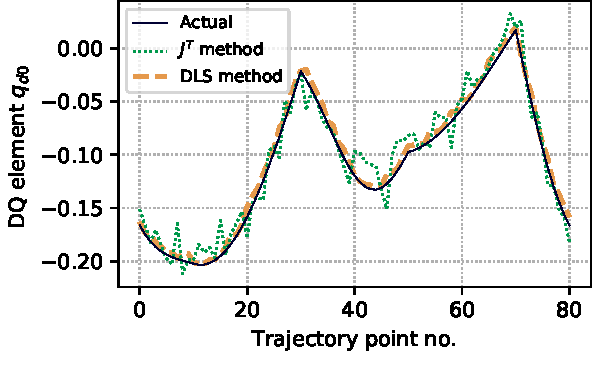
\includegraphics[width=0.4 \textwidth]{./imgs/trajectoryq4c.pdf}  }
	\hfill
	\subfloat{ 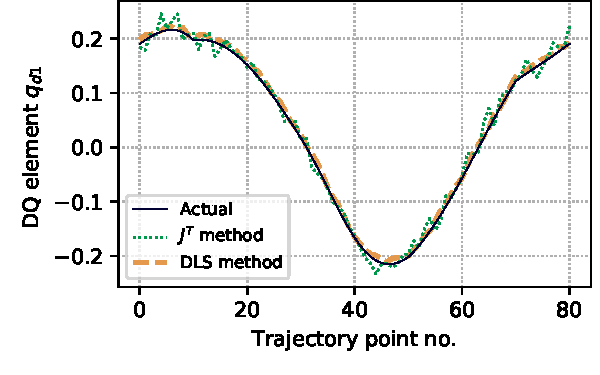
\includegraphics[width=0.4 \textwidth]{./imgs/trajectoryq5c.pdf}  }
	\caption{ Comparison of DQ elements ($q_{d0}$ and $q_{d1}$) traced by $J^T$ and DLS IK models \cite{fernandez2015}}  \label{fig:dqelements}
\end{figure}



\begin{table}[h] \centering
	\caption{ Frame transformations carried out using \cite{lentin2015} } \label{tab:screwmotions}
	\begin {tabular}[h]	{| c | c  c |}	 \hline 
	%	\begin {tabular}[h]	{| c | p{0.35\textwidth} | p{0.35\textwidth} |}	 \hline		
	\shortstack{Frame \\ transformation}   &   $\left\lbrace i-1 \right\rbrace$ to $\left\lbrace i' \right\rbrace$   &   $\left\lbrace i' \right\rbrace$ to $\left\lbrace i \right\rbrace$ \\ \hline
	Rotation angle $ \theta $   &   $ \theta_i $   &   $ \alpha_i $ \\ \hline
	Rotation axis $ \hat{\vec{u}} $   &   $ ( 0, 0, 1 ) $   &   $ ( 1, 0, 0 ) $ \\ \hline
	\shortstack{Translation \\ direction $ \vec{t} $ }  &   $ ( 0, 0, d_i ) $   &   $ ( a_i, 0, 0 ) $ \\ \hline
	$ \hat{\vec{u}} \cdot \vec{t} $   &   $ d_i $   &   $ a_i $ \\ \hline
	$ \hat{\vec{u}} \times \vec{t} $   &   $ 0 $   &    $ 0 $ \\ \hline
	\shortstack{Transformation \\ DQ} & 
	\shortstack {  $ \underline{q}^Z = \left[ C_\theta, \, 0, \, 0, \, S_\theta \right] +  \qquad $   \\   $ \qquad \epsilon \left[ -  D S_\theta, \, 0, \, 0, \, D C_\theta \right] $   }   &
	\shortstack {  $ \underline{q}^X = \left[ C_\alpha, S_\alpha, 0, 0 \right] +  \qquad $   \\   $ \qquad \epsilon \left[ - A S_\alpha,  A C_\alpha, 0, 0 \right] $  }  \\ \hline \end{tabular} 
\end{table}










\bibliographystyle{unsrt}
\bibliography{mybibliography} 

\end{document}